\chapter{Drive test study July 2017}\label{app:drive_test_study_2017}

A drive test of the Technical University of Denmark campus area was performed by students under Henrik L. Christiansen. The data obtained have later been utilized for research related to path loss modelling. The drive test was conducted using professional drive test equipment supplied by \gls{r_and_s}. More specifically, the equipment utilized was a TSMW \cite{Manual2017}, along with the software ROMES \cite{ROMESmanual}. Two antennas was mounted on top of the vehicle, each with independent RF front-ends for parallel measurements.

The \gls{rsrp} and \gls{rsrq} as a function of antenna separation distance is shown in figure \ref{fig:drive_test_2017_example}.
The area covered by this study is visualized in Fig. \ref{fig:drivetest_area} along with the \gls{rsrp} measurement. All measurements are added on-top of each other, and the location of the base station is shown.

\begin{marginfigure}
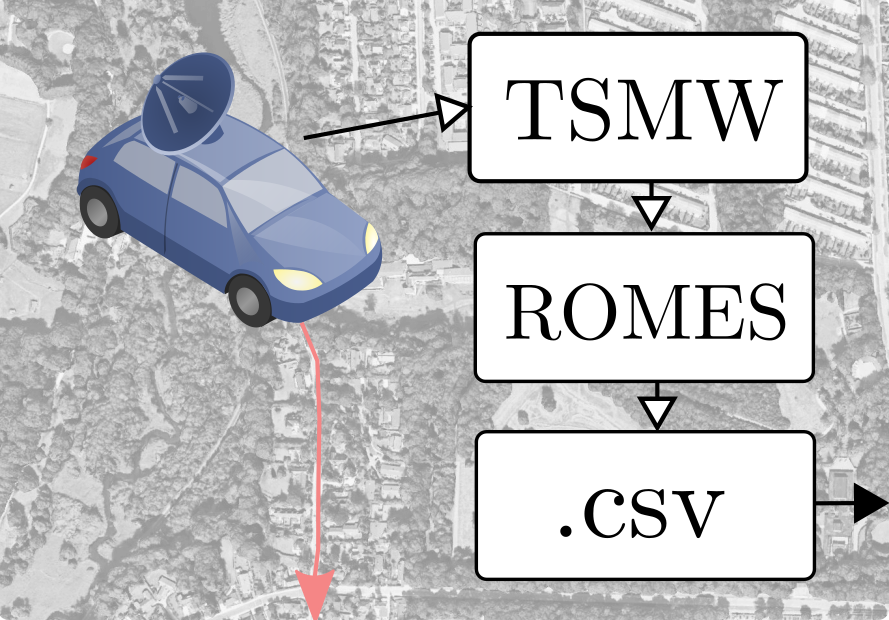
\includegraphics[]{appendix/figures/drive_test_equipment.png}
\caption{The TSMW was used in conjunction with the ROMES software suite. This offers a replayable drive test, and allows for an export of desired metrics. Such as LTE reference parameters \gls{rsrp} etc.}
\end{marginfigure}

A majority of LTE bands were scanned. However, two particular frequencies of the resulting drive test were used for the creation of the data set in \cite{1xf4-eg98-19}. The distribution of the samples can be observed in Table \ref{tab:drive_test_2017}.

\begin{table}[]
\centering
\begin{tabular}{@{}ll@{}}
\toprule
Frequency {[}MHz{]} & Samples                      \\ \midrule
811                 & 33970                        \\
2630                & 23616                        \\ \midrule
Total               & 57586      \\ \bottomrule
\end{tabular}
\caption{The amount of measurements at 811 and 2630 MHz}\label{tab:drive_test_2017}
\end{table}


\begin{figure*}
    \centering
    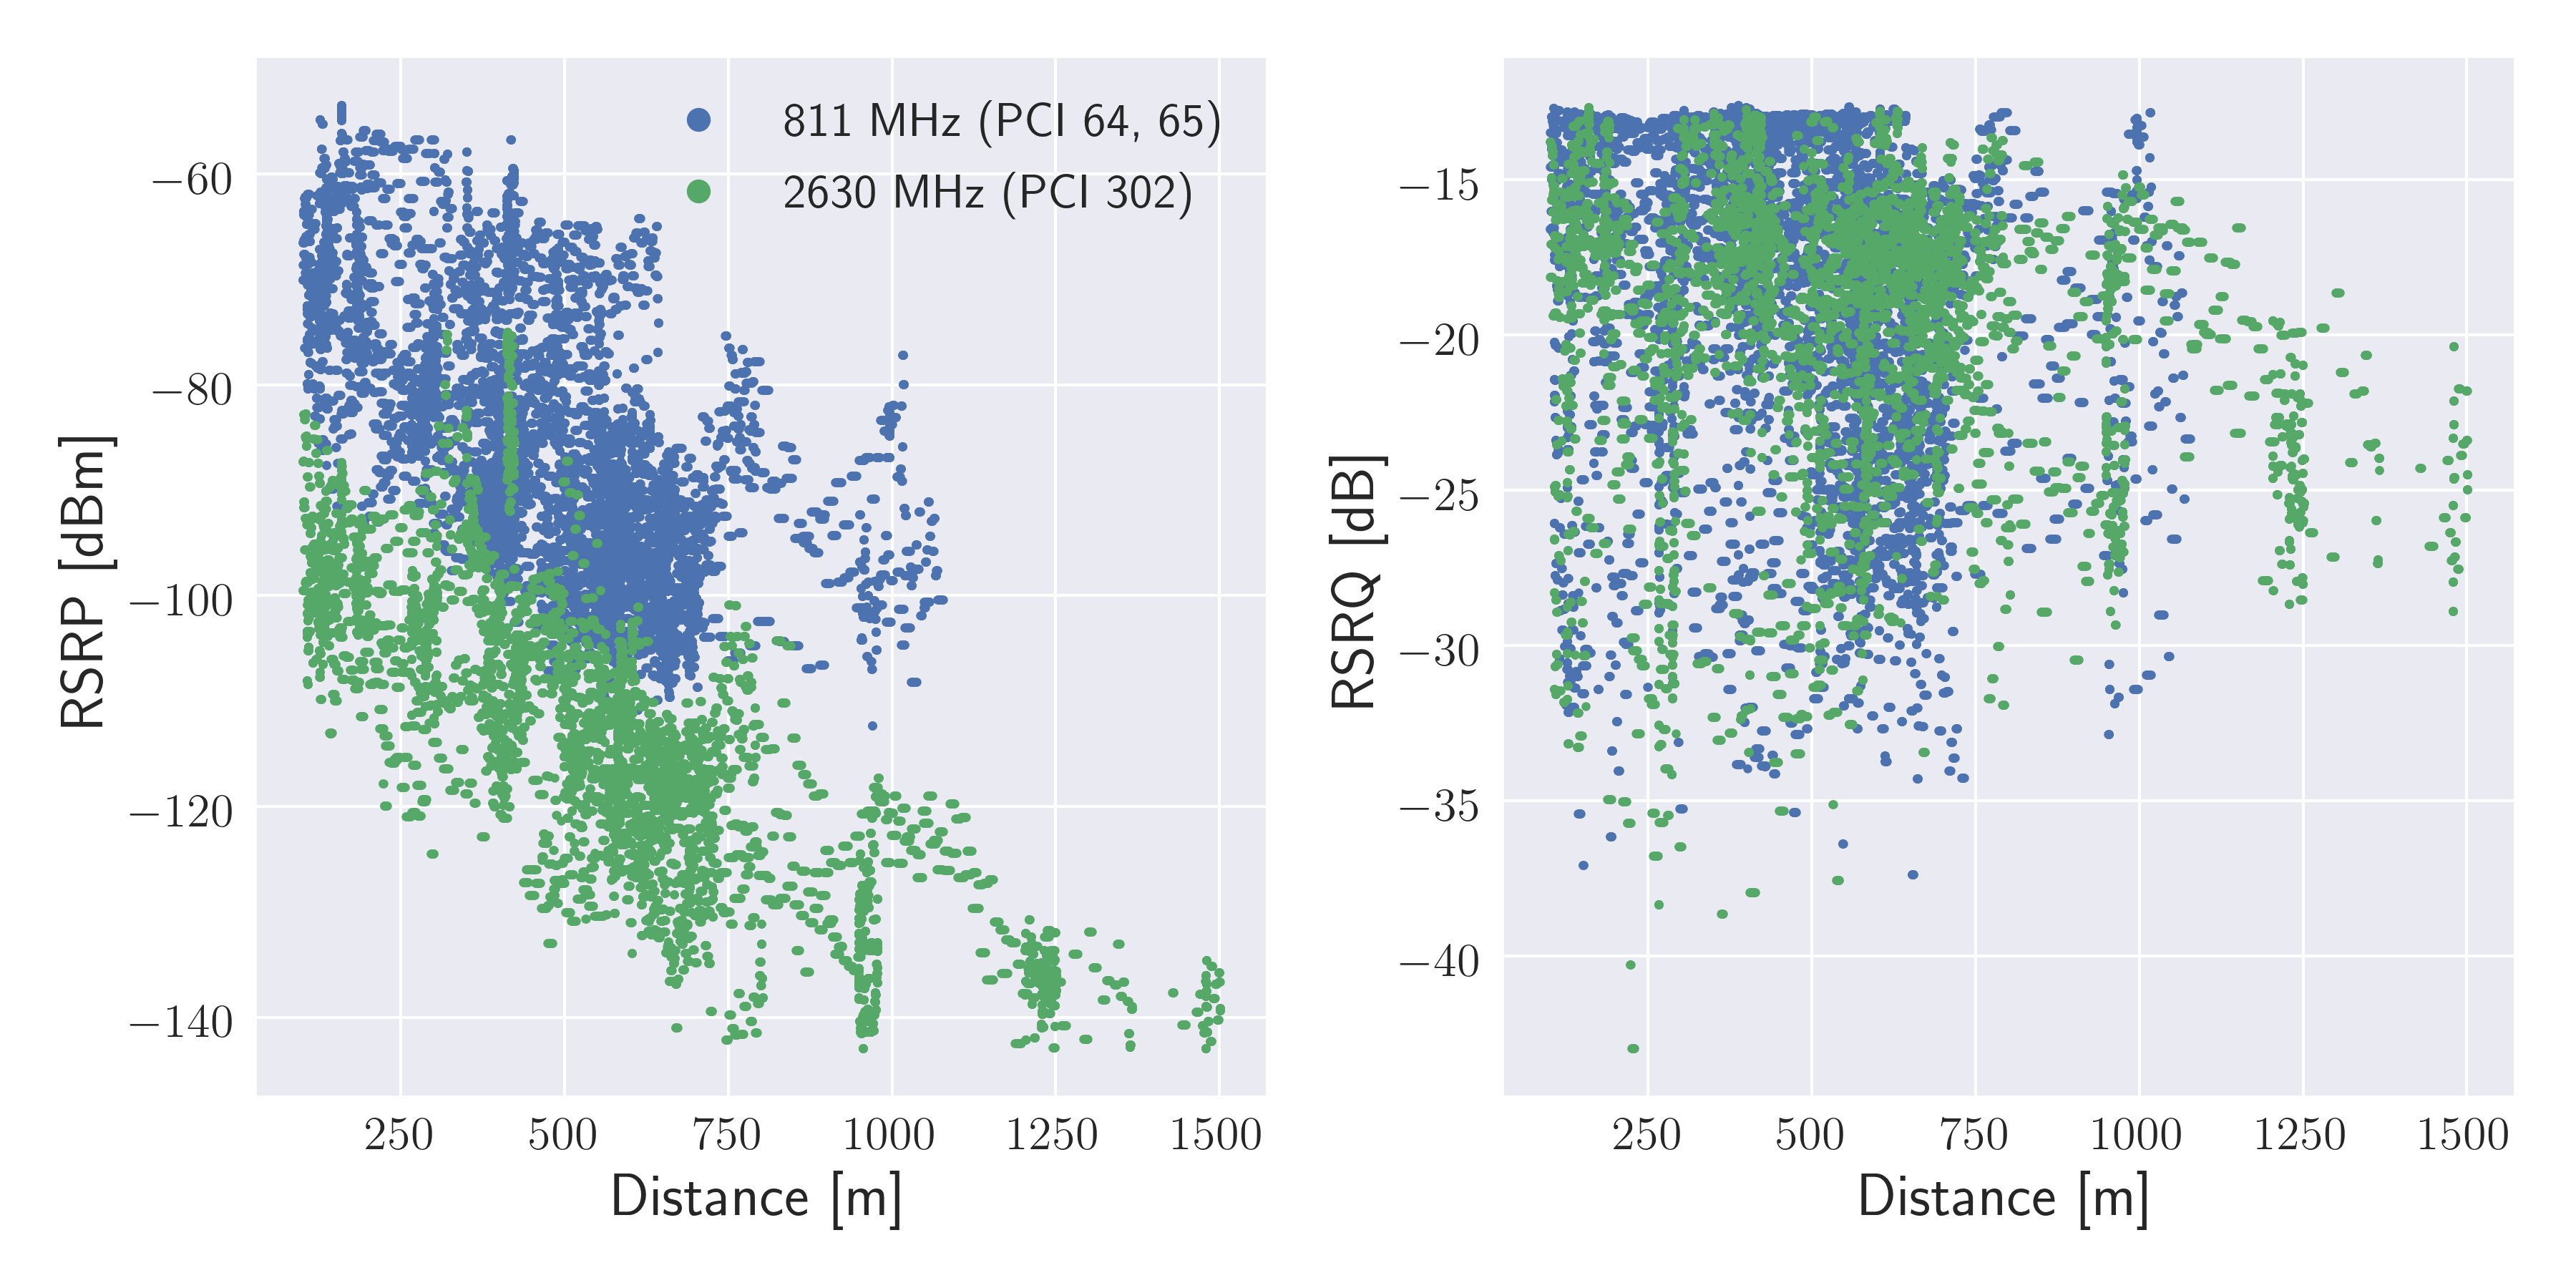
\includegraphics[width=0.8\textwidth]{appendix/figures/drive_test_2017_811_2630_example.png}
    \caption{\gls{rsrp} and \gls{rsrq} measurements over increased antenna separation distance between transmitter and receiver}
    \label{fig:drive_test_2017_example}
\end{figure*}

\begin{figure*}
    \centering
    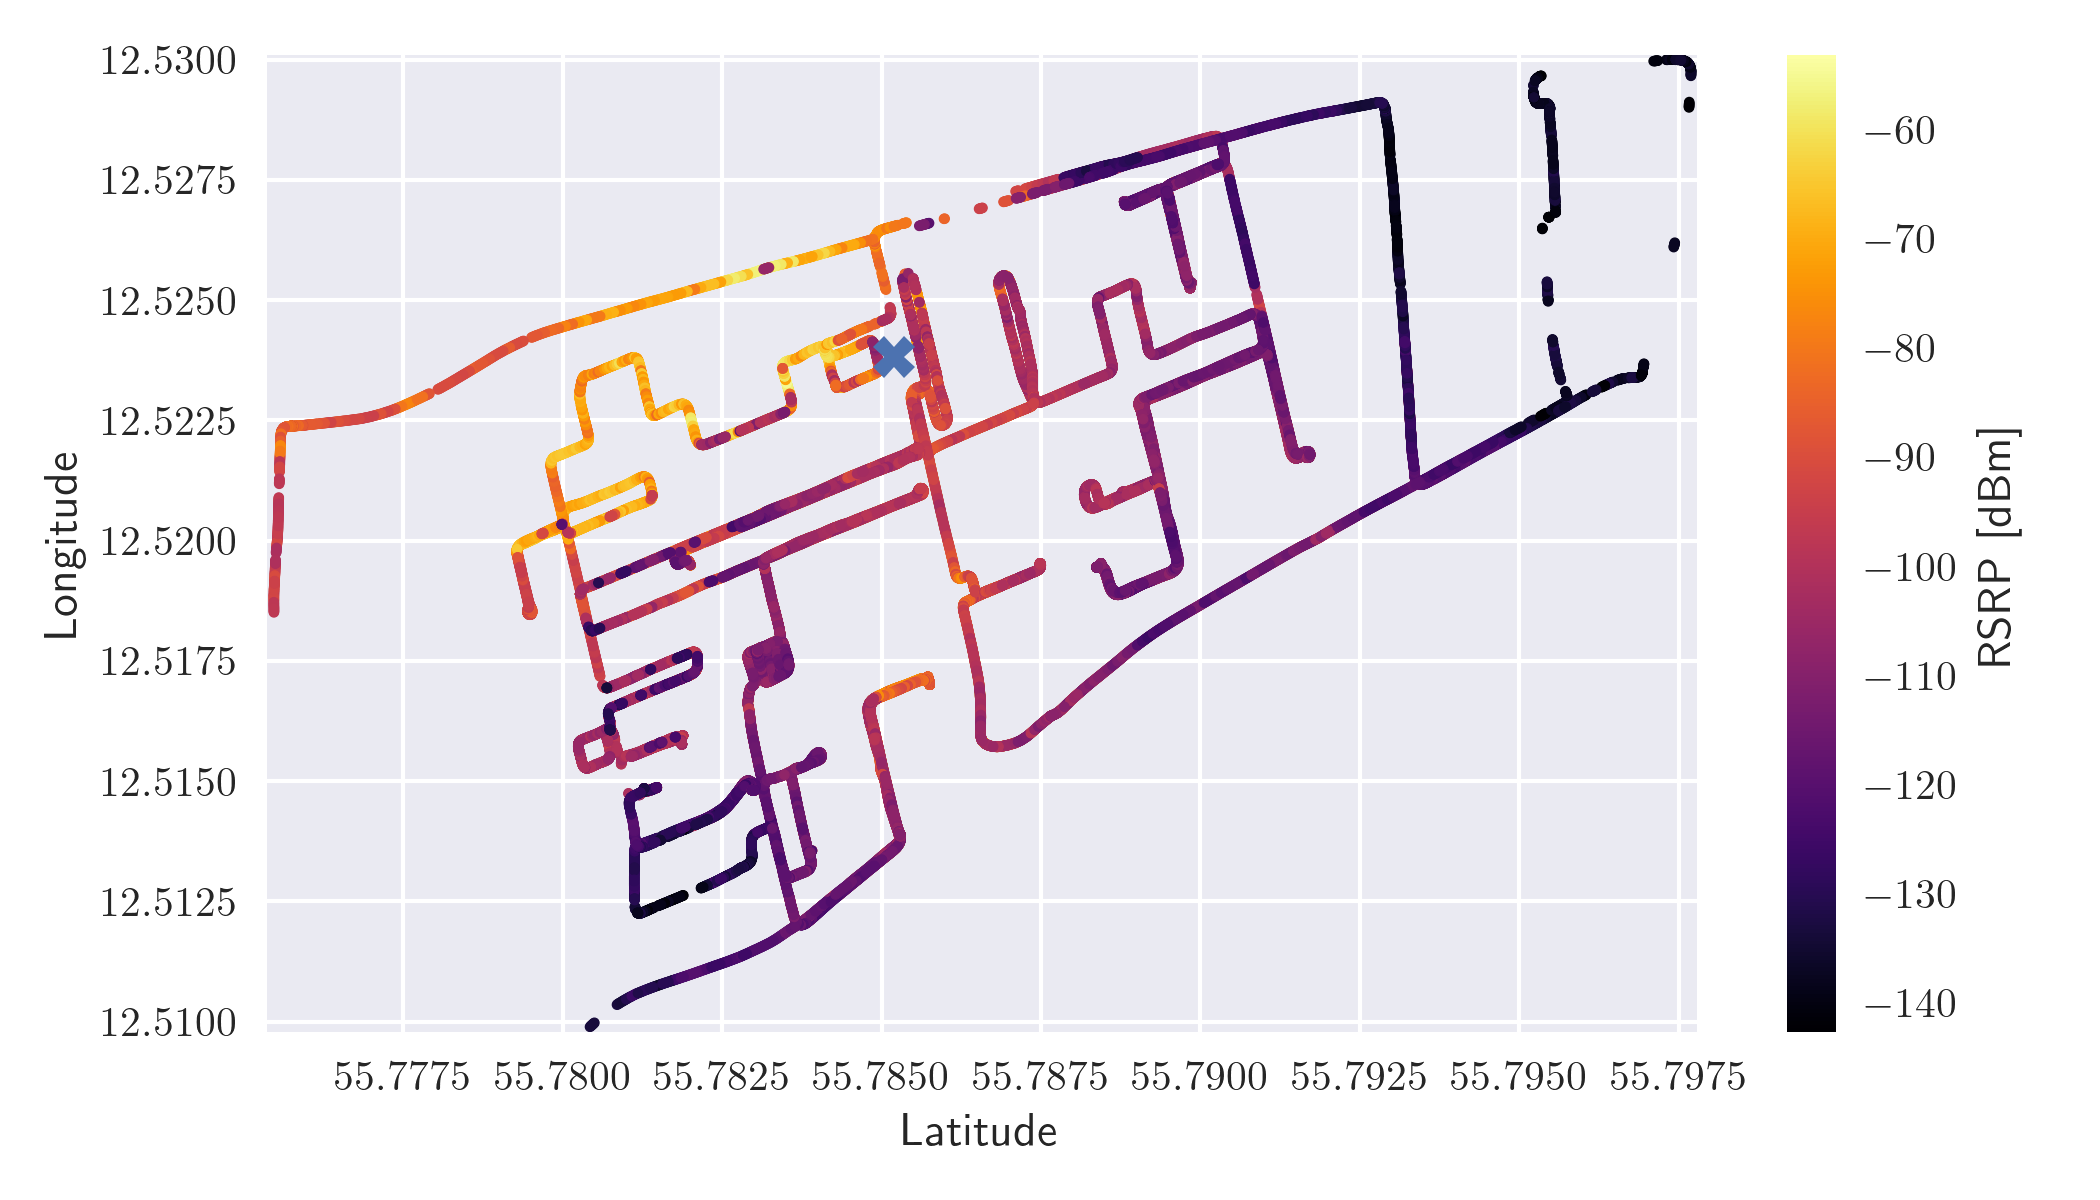
\includegraphics[width=0.7\textwidth]{appendix/figures/drivetest_2017_scatter.png}
    \caption{All \gls{rsrp} measurements along with the location of the base station.}
    \label{fig:drivetest_area}
\end{figure*}


\chapter{Drive test study February 2020}\label{app_drive_test_study_2020}

A drive study was completed in early 2020, and can be found at \cite{keyt-8g44-20}. The area of the Technical University of Denmark was driven in a similar fashion as the 2017 study. A \gls{r_and_s} TSMW \cite{Manual2017}, along with the software ROMES \cite{ROMESmanual} was utilized for obtaining the measurements. The amount of frequencies scanned in the data set can be found in Table \ref{tab:drive_test_2020}.

Examples of \gls{rsrp} measurements and the measured area can be found in Fig. \ref{fig:drive_test_2020_scatter} for a multitude of \glspl{pci}. The frequencies shown are $811$ (63, 64, 65) and $2630$ (294, 298, 302) MHz, however, separated per sector of a single site. 

\begin{margintable}
\begin{tabular}{@{}ll@{}}
\toprule
Frequency {[}MHz{]} & Samples                      \\ \midrule
796                 & 1208                         \\
811                 & 1024                         \\
1815                & 2612                         \\
1835                & 2788                         \\
1870                & 3397                         \\
2160                & 3428                         \\
2630                & 2330                         \\
2645                & 4301                         \\
2660                & 1789                         \\ \midrule
Total               & 22877	 \\ \bottomrule
\end{tabular}
\caption{Measured frequencies and the resulting amount of measurements}\label{tab:drive_test_2020}
\end{margintable}

\begin{figure*}
    \centering
    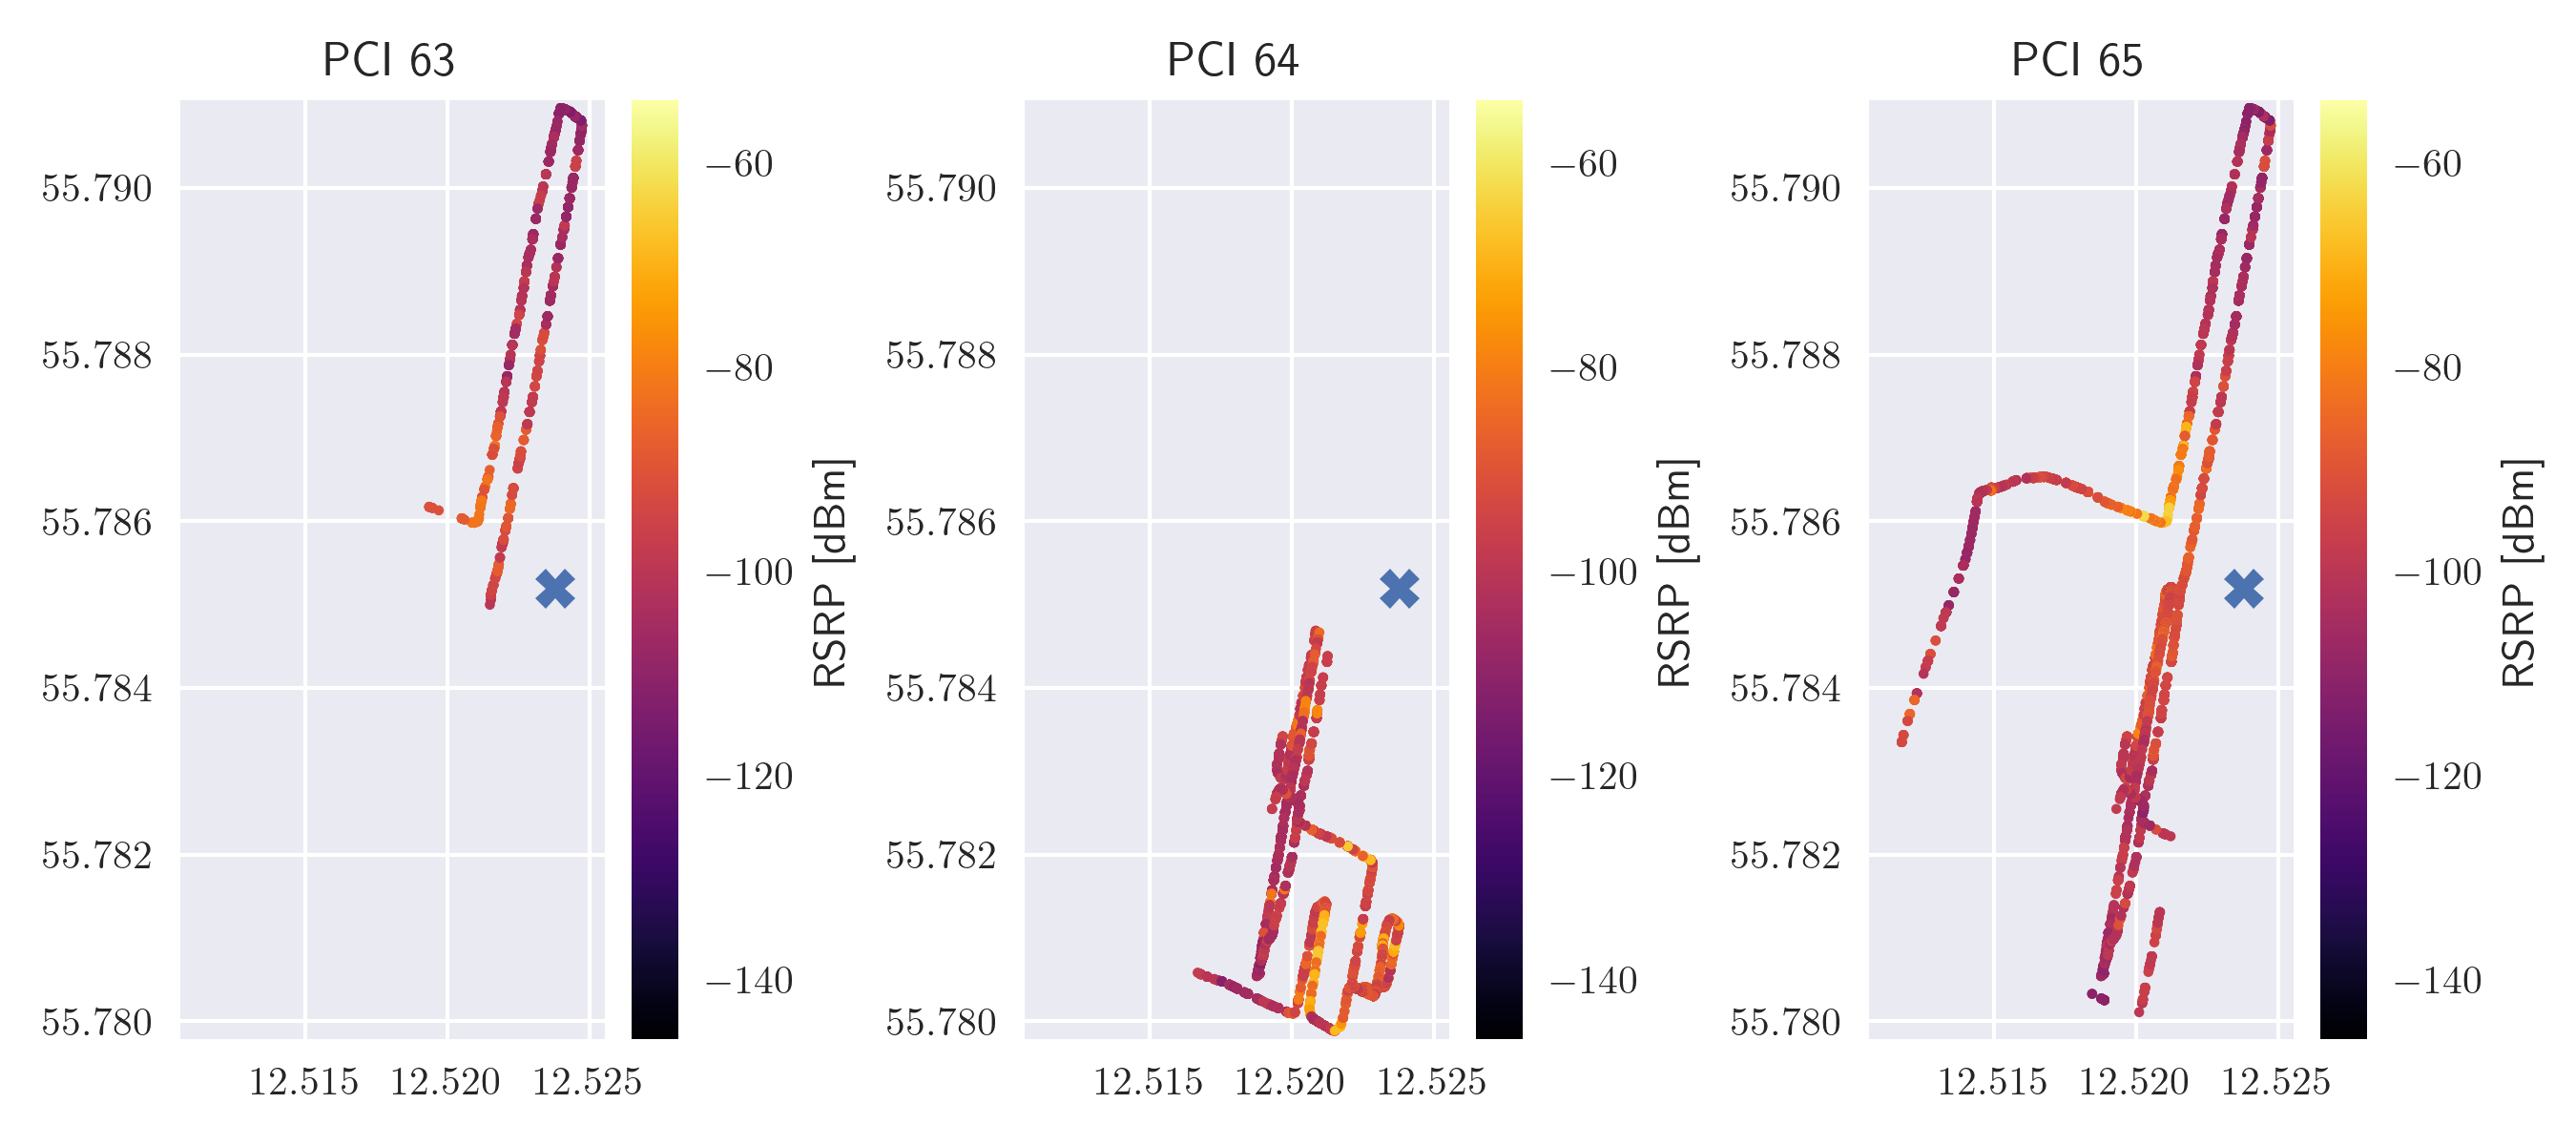
\includegraphics[width=0.95\textwidth]{appendix/figures/pci_63_64_65_scatter.png}
    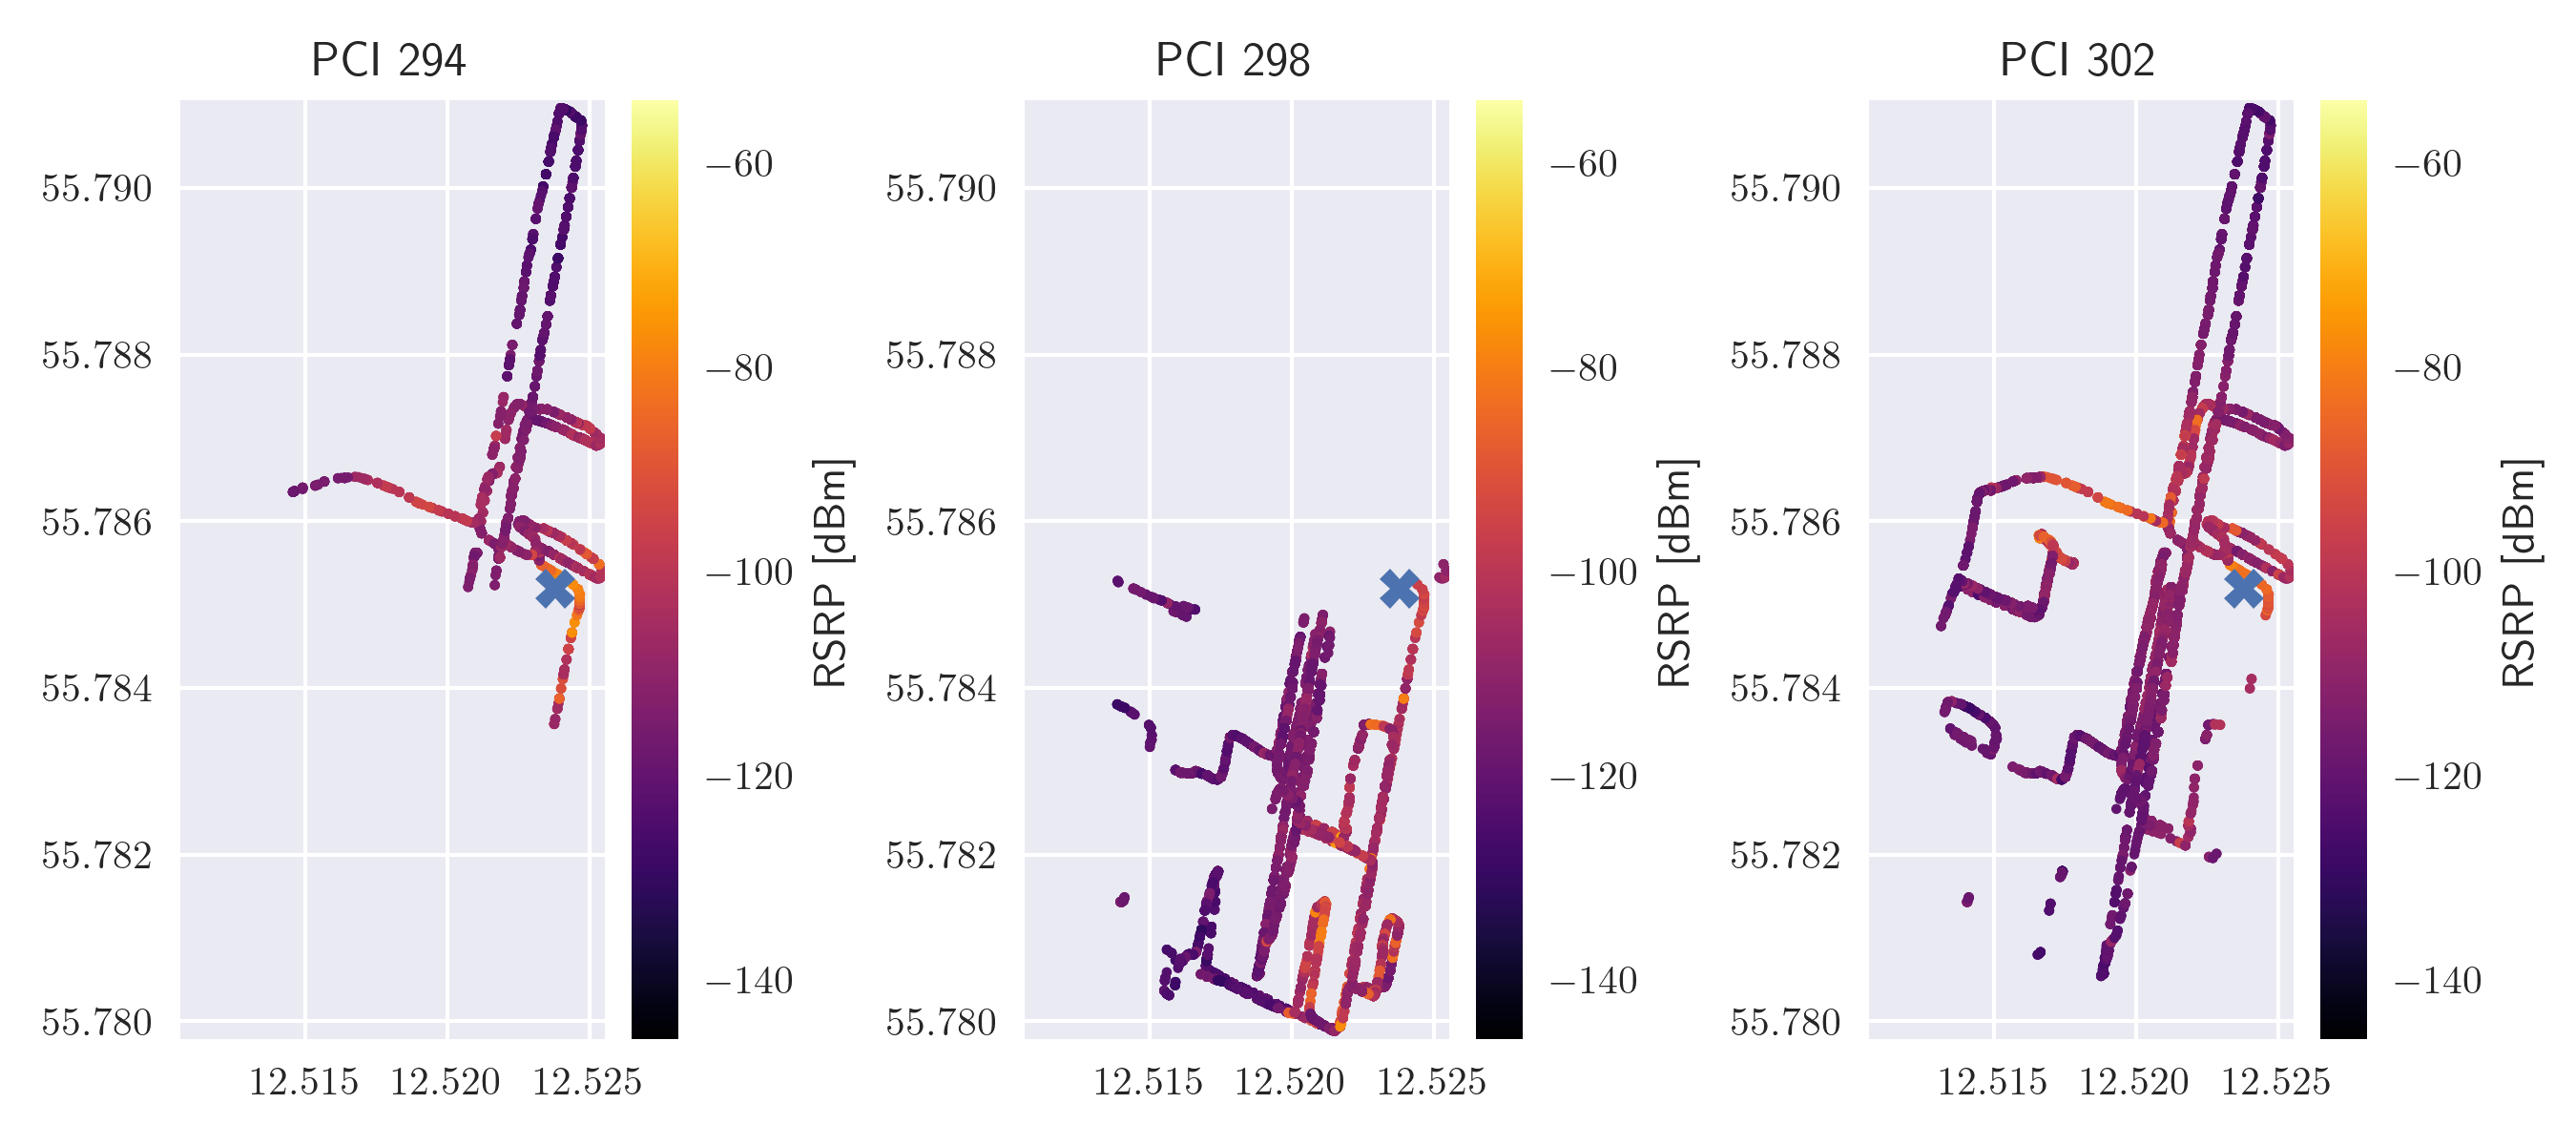
\includegraphics[width=0.95\textwidth]{appendix/figures/pci_294_298_302_scatter.png}
    \caption{\gls{rsrp} Measurements of the driven area for two sites operating at different frequencies of 811 and 2630 MHz.}
    \label{fig:drive_test_2020_scatter}
\end{figure*}
